\chapter{Растворы, диаграммы состояния и водород в цирконии}

\section{Идеальный раствор: энтропия перемешивания}

Возьмём $N$ узлов решётки и рассадим на них $N_B = XN$ атомов сорта $B$ и $N_A = (1-X)N$ атомов $A$. Число
различимых расстановок $W = N!/(N_A!\,N_B!)$. По Больцману энтропия $S = k_B\ln W$; с формулой Стирлинга
$\ln N! \approx N\ln N - N$ получаем на моль
\begin{equation}
\Delta S_{\text{mix}} = -R\,\bigl[X\ln X + (1-X)\ln(1-X)\bigr] .
\end{equation}
Если атомы $A$ и $B$ «безразличны» друг к другу (энергия связи $A$--$B$ равна средней из $A$--$A$ и $B$--$B$),
теплота смешения равна нулю, и
\begin{equation}
\Delta G_{\text{mix}} = RT\,\bigl[X\ln X + (1-X)\ln(1-X)\bigr] < 0 .
\end{equation}
Это \textbf{идеальный раствор}. Смешение выгодно всегда, при любом составе: энтропия выигрывает «бесплатно».

\begin{idea}
У функции $X\ln X$ производная при $X\to 0$ уходит в $-\infty$. Значит, \emph{первые} атомы примеси растворяются
с огромным выигрышем энтропии. Поэтому абсолютно чистых веществ не бывает и растворимость любой примеси, пусть
крошечная, всегда больше нуля.
\end{idea}

\section{Регулярный раствор: когда соседи не безразличны}

Пусть энергии связей различаются. В простейшей модели каждый атом взаимодействует только с $z$ ближайшими
соседями, а расстановка остаётся случайной. Тогда теплота смешения
\begin{equation}
\Delta H_{\text{mix}} = \Omega X(1-X),\qquad
\Omega = N_A z\Bigl[\eps_{AB} - \tfrac12(\eps_{AA}+\eps_{BB})\Bigr],
\end{equation}
и $\Delta G_{\text{mix}} = \Omega X(1-X) + RT[X\ln X + (1-X)\ln(1-X)]$. Знак $\Omega$ решает всё
(рис.~\ref{fig:f2_mixing}):
\begin{itemize}
\item $\Omega < 0$: разноимённые соседи выгодны, раствор ещё устойчивее идеального, при низких $T$ возможно упорядочение;
\item $\Omega > 0$: выгоднее одноимённые соседи. Пока $T$ высока, энтропия держит раствор однородным; при
  $\Omega/RT > 2$ на кривой $G(X)$ появляются две ямы --- раствор хочет разделиться на две фазы.
\end{itemize}

\fig{f2_mixing}{а) Энергия смешения регулярного раствора в единицах $RT$ при разных $\Omega/RT$. При
$\Omega/RT > 2$ появляется двойная яма. б) Для $\Omega/RT = 2.5$: энтальпия (красная) против смешения,
энтропийный член (синий) --- за; сумма (чёрная) имеет два минимума.}

Химический потенциал компонента $B$ в регулярном растворе
\begin{equation}
\mu_B = G_B^0 + \Omega(1-X)^2 + RT\ln X .
\end{equation}
Для разбавленного раствора ($X\to 0$) член $\Omega(1-X)^2\to\Omega$ --- константа, и
\begin{keyf}[Разбавленный раствор]
\[
\mu_B \approx \mu_B^{\infty} + RT\ln X .
\]
\end{keyf}
Это закон Генри: в разбавленном растворе химический потенциал растёт как логарифм концентрации, что бы ни
происходило с атомами в деталях. Водород в $\alpha$-цирконии --- как раз такой случай: даже 600~ppm --- это
5~ат.\,\%. Вся термодинамика растворимости гидридов держится на одной этой формуле.

\section{Расслоение: бинодаль, спинодаль, общая касательная}

Если кривая $G(X)$ имеет две ямы, раствор состава $X_0$ между ними может понизить энергию, распавшись на две
части с составами $X_1$ и $X_2$. Энергия смеси лежит на \emph{хорде}, соединяющей точки кривой, и наилучшая
хорда --- \textbf{общая касательная} (рис.~\ref{fig:f2_gap}б). В точках касания одинаков наклон
$\partial G/\partial X$; это и есть условие равенства химических потенциалов обоих компонентов в двух фазах.

\begin{keyf}[Общая касательная и правило рычага]
Равновесные составы фаз $X_1$, $X_2$ --- точки касания общей касательной. Доли фаз в сплаве состава $X_0$:
\[
f_2 = \frac{X_0 - X_1}{X_2 - X_1},\qquad f_1 = 1 - f_2 .
\]
\end{keyf}

Если провести такое построение при каждой температуре, точки касания образуют \textbf{бинодаль} --- границу
двухфазной области на диаграмме состояния (рис.~\ref{fig:f2_gap}а). Внутри неё есть ещё одна линия ---
\textbf{спинодаль}, где кривизна $\partial^2G/\partial X^2$ меняет знак:
\begin{equation}
\frac{\partial^2 G}{\partial X^2} = -2\Omega + \frac{RT}{X(1-X)} = 0
\quad\Rightarrow\quad X(1-X) = \frac{RT}{2\Omega},\qquad T_c = \frac{\Omega}{2R}.
\end{equation}

\fig{f2_gap}{а) Купол расслоения регулярного раствора: бинодаль (чёрная) и спинодаль (красная пунктирная).
Между ними раствор метастабилен --- для распада нужно зарождение; внутри спинодали распад идёт без барьера.
б) Сечение при $T = 0.7\,T_c$: общая касательная (золотая) и точки перегиба (красные квадраты).}

\begin{idea}
Почему между бинодалью и спинодалью нужен барьер? Там кривая $G(X)$ выпукла вниз: \emph{малое} расслоение
(состав чуть больше и чуть меньше среднего) энергию повышает. Выигрыш появляется, только если сразу возникает
кусочек совсем другого состава --- зародыш новой фазы. Внутри спинодали кривая выпукла вверх, и любое малое
колебание состава растёт само. Выпадение гидридов --- случай первого типа: гидрид по составу и решётке
совсем не похож на раствор, поэтому без зарождения он не появится.
\end{idea}

\section{Растворимость второй фазы}

Теперь самое важное для нас. Пусть вторая фаза --- почти стехиометрическое соединение, например гидрид
$\mathrm{ZrH}_x$ с $x \approx 1.6$. Его кривая $G(X)$ --- узкая глубокая яма около $X_\delta \approx 0.62$
(рис.~\ref{fig:f2_tangent}). Общая касательная к ней и к кривой твёрдого раствора касается раствора в точке
$X_e$ --- это и есть \textbf{предел растворимости}.

\begin{figure}[htbp]\centering
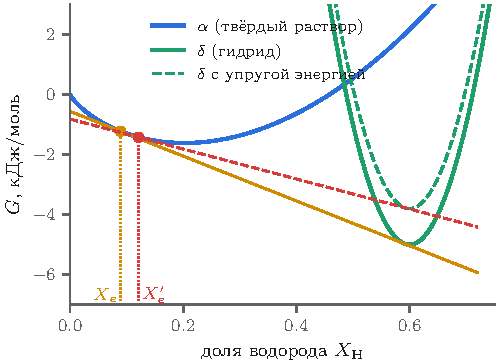
\includegraphics[width=0.62\linewidth]{f2_tangent}
\caption{Растворимость соединения в твёрдом растворе (схема). Общая касательная (золотая) к раствору $\alpha$ и
гидриду $\delta$ касается раствора в точке $X_e$. Если энергия гидрида выше (пунктир: упругая энергия
несоответствия, малый размер), касательная круче и растворимость $X_e'$ больше.}
\label{fig:f2_tangent}
\end{figure}

Посчитаем $X_e$. В равновесии химический потенциал водорода одинаков в растворе и в гидриде. В разбавленном
растворе $\mu_{\mathrm H}^\alpha = \mu_{\mathrm H}^{\infty} + RT\ln X$; в гидриде он почти не зависит от состава.
Пусть $\Delta G^0 = \Delta H^0 - T\Delta S^0$ --- изменение энергии при переводе моля водорода из гидрида в
раствор (при стандартной концентрации). Тогда $RT\ln X_e = -\Delta G^0$, и
\begin{keyf}[Предел растворимости]
\[
X_e = \exp\!\Bigl(\frac{\Delta S^0}{R}\Bigr)\exp\!\Bigl(-\frac{\Delta H^0}{RT}\Bigr) \equiv A\,e^{-Q/RT}.
\]
\end{keyf}
В координатах $\ln C$ против $1/T$ это прямая; её наклон даёт теплоту растворения $Q$, отрезок --- энтропийный
множитель $A$. Именно так и записывают экспериментальные линии растворимости водорода в цирконии.

\section{Водород в цирконии: две линии вместо одной}

Опыт (дифференциальная сканирующая калориметрия, дилатометрия, дифракция) даёт не одну линию растворимости, а
две (рис.~\ref{fig:f2_tss}):
\begin{itemize}
\item \textbf{TSSD} (terminal solid solubility for dissolution) --- при нагреве гидриды полностью растворяются,
  когда концентрация в растворе достигает этой линии;
\item \textbf{TSSP} (for precipitation) --- при охлаждении гидриды начинают выпадать заметно ниже, при концентрации
  на этой линии.
\end{itemize}

\fig{f2_tss}{а) Пределы растворимости водорода в сплаве Э635: растворение (TSSD) и выпадение (TSSP), линии
вида $\lg C = b - k\cdot 1000/T$ по данным ДСК (Плясов и др., 2023). Пунктир --- путь образца со 160~ppm:
при нагреве гидриды растворяются полностью при 394\degC, при охлаждении начинают выпадать только при 311\degC.
б) Те же линии в аррениусовых координатах: прямые с теплотами около 43 и 32~кДж/моль.}

Между линиями --- полоса гистерезиса шириной около 80\degC. Откуда она? Вернёмся к рис.~\ref{fig:f2_tangent}.
Новому гидриду, чтобы появиться, приходится «заплатить» сверх табличной энергии соединения:
\begin{itemize}
\item \textbf{упругую энергию несоответствия}: гидрид объёмнее циркония на 17\,\%, и матрица вокруг него
  деформирована (глава~5);
\item \textbf{работу пластической аккомодации}: часть несоответствия снимается пластическим течением, которое тоже
  требует работы (глава~7);
\item \textbf{энергию межфазной границы} и вообще барьер зарождения (глава~6).
\end{itemize}
Каждая такая добавка $\Delta g$ (на моль водорода) поднимает кривую гидрида, и растворимость, с которой он
равновесен, растёт в $e^{\Delta g/RT}$ раз:
\begin{equation}
\frac{C_\TSSP}{C_\TSSD} = \exp\Bigl(\frac{\Delta g}{RT}\Bigr)
\quad\Rightarrow\quad
\Delta g = RT\ln\frac{C_\TSSP}{C_\TSSD} .
\end{equation}
При растворении всё наоборот: старый гидрид уже окружён релаксированной (пластически деформированной) матрицей,
лишней энергии у него почти нет, и он растворяется близко к «истинному» равновесию.

\begin{zrbox}
Для Э635 при 300\degC: $C_\TSSD \approx 45$~ppm, $C_\TSSP \approx 141$~ppm, отношение 3.1. Значит, на линии
выпадения раствор пересыщен на $\Delta g = RT\ln 3.1 \approx 5.5$~кДж на моль водорода. В главе~5 мы увидим, что
одна только упругая энергия тонкой пластинки гидрида около 3~кДж/моль~H --- того же порядка. Остальное
--- пластичность и барьер зарождения. Линия TSSP к тому же частично \emph{кинетическая}: она смещается со скоростью
охлаждения и с тем, до какой температуры образец нагревали (сохранились ли следы старых гидридов).
\end{zrbox}

\section{Диаграмма Zr--H со стороны циркония}

Полная диаграмма Zr--H сложна: несколько гидридов ($\gamma$-ZrH, $\delta$-ZrH$_{\sim1.6}$, $\varepsilon$-ZrH$_2$),
высокотемпературная $\beta$-фаза, эвтектоид. Для оболочек важен только угол со стороны циркония
(рис.~\ref{fig:f2_zrh}):
\begin{itemize}
\item $\alpha$ --- твёрдый раствор водорода в ГПУ цирконии;
\item $\alpha+\delta$ --- раствор плюс гидрид; граница --- линия растворимости (TSSD);
\item $\beta$ --- ОЦК цирконий; водород её стабилизирует, поэтому область $\alpha+\beta$ клином уходит вниз;
\item эвтектоид при $\approx 550$\degC: $\beta \to \alpha + \delta$. Растворимость в $\alpha$ там максимальна,
  $\approx 6$~ат.\,\% (около 690~ppm).
\end{itemize}

\begin{figure}[htbp]\centering
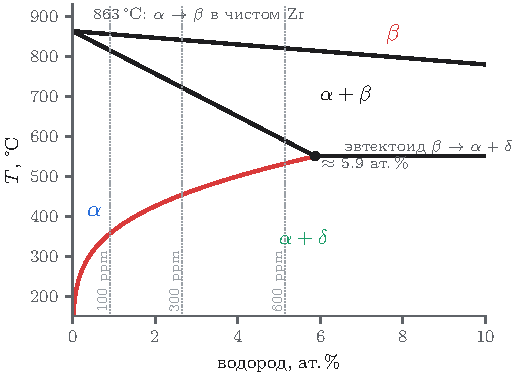
\includegraphics[width=0.6\linewidth]{f2_zrh}
\caption{Угол диаграммы Zr--H со стороны циркония (схема; сольвус $\alpha/(\alpha+\delta)$ --- по линии TSSD,
остальные границы условно прямыми). Вертикальные пунктиры --- 100, 300 и 600~ppm водорода.}
\label{fig:f2_zrh}
\end{figure}

\begin{warnbox}
Сплавы (Nb, Sn, Fe, O) немного сдвигают линии, а линия выпадения зависит от режима охлаждения. Поэтому для
конкретного материала линии берут из его собственных измерений, а не из общей диаграммы.
\end{warnbox}

\section{Сколько выпадает гидрида}

По правилу рычага при комнатной температуре почти весь водород сидит в гидриде (растворимость там --- доли ppm).
В $\delta$-ZrH$_{1.66}$ водорода $\approx 1.8$\,\% по массе (18\,000~ppm). Значит, при 160~ppm массовая доля
гидрида $160/18\,000 \approx 0.9\,\%$, а объёмная --- около 1\,\% (гидрид менее плотен). На шлифе после травления
гидриды кажутся занимающими 7--12\,\% площади --- травление сильно расширяет их следы. Об этом стоит помнить,
сравнивая снимки с расчётом.

\begin{exercise}
Выведите выражение для $\mu_B$ регулярного раствора, продифференцировав $G = (1-X)G_A + XG_B + \Delta G_{\text{mix}}$.
Проверьте, что при $X\to 0$ получается закон Генри.
\end{exercise}

\begin{exercise}
Для линии $\lg C = 5.56 - 2240/T$ найдите теплоту растворения $Q$ в кДж/моль и температуру полного растворения
для 100, 300 и 600~ppm.
\end{exercise}

\begin{exercise}
Пользуясь линиями Э635, постройте $\Delta g(T) = RT\ln(C_\TSSP/C_\TSSD)$ от 200 до 400\degC. Растёт она или падает с
температурой? Как это согласуется с тем, что пластичность легче при высокой температуре?
\end{exercise}

\begin{exercise}
Образец с 300~ppm нагрели до 400\degC. Сколько водорода осталось в нерастворённых гидридах? При какой температуре
начнётся выпадение при охлаждении?
\end{exercise}
